\section{Disjoint Set Union: Path Compression}

\begin{frame}
\frametitle{Disjoint Set Union: Path Compression}
Let's change the definition of the parent array.
\begin{block}{Definition: Parent Array}
    parent[u] := root of the component of vertex $u$.
\end{block}

\begin{center}
\begin{tikzpicture}
[  
    level 1/.style={sibling distance=25mm},
    level 2/.style={sibling distance=15mm},
    edge from parent/.style={thick}
]
    \begin{scope}[edge from parent/.style={draw=red}]
        \node [draw, circle, red] {1}
            child {node [draw, circle, red] {3}}
            child {
                node [draw, circle, red] {2}
                child {node [draw, circle, red] {4}}
            };
    \end{scope}
    
    \begin{scope}[edge from parent/.style={draw=orange}]
        \node [draw, circle, orange] at (6,0) {5}
            child {
                node [draw, circle, orange] {7}
                child {node [draw, circle, orange] {6}}
                child {node [draw, circle, orange] {8}}
            };
    \end{scope}
\end{tikzpicture}
\end{center}

\begin{center}
\begin{tabular}{|c||c|c|c|c|c|c|c|c|}
    \hline
    index & 1 & 2 & 3 & 4 & 5 & 6 & 7 & 8\\
    \hline
    \hline
    parent & 1 & 1 & 1 & 2 & 5 & 7 & 5 & 7\\
    \hline
\end{tabular}
\end{center}
\end{frame}

\begin{frame}
\frametitle{Disjoint Set Union: Path Compression}
Let's change the definition of the parent array.
\begin{block}{Definition: Parent Array}
    parent[u] := root of the component of vertex $u$.
\end{block}

\begin{center}
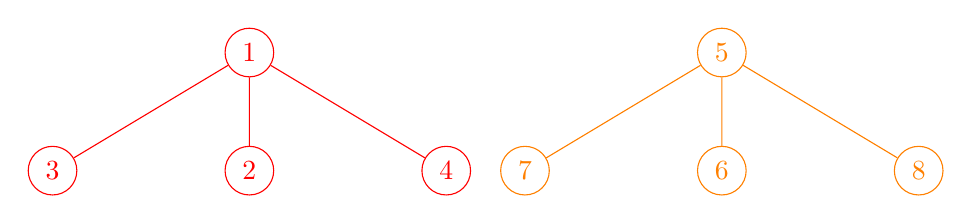
\begin{tikzpicture}
[  
    level 1/.style={sibling distance=25mm},
    level 2/.style={sibling distance=15mm},
    edge from parent/.style={thick}
]
    \begin{scope}[edge from parent/.style={draw=red}]
        \node [draw, circle, red] {1}
            child {node [draw, circle, red] {3}}
            child {node [draw, circle, red] {2}}
            child {node [draw, circle, red] {4}};
    \end{scope}
    
    \begin{scope}[edge from parent/.style={draw=orange}]
        \node [draw, circle, orange] at (6,0) {5}
            child { node [draw, circle, orange] {7}}
            child {node [draw, circle, orange] {6}}
            child {node [draw, circle, orange] {8}};
    \end{scope}
\end{tikzpicture}
\end{center}

\begin{center}
\begin{tabular}{|c||c|c|c|c|c|c|c|c|}
    \hline
    index & 1 & 2 & 3 & 4 & 5 & 6 & 7 & 8\\
    \hline
    \hline
    parent & 1 & 1 & 1 & 1 & 5 & 5 & 5 & 5\\
    \hline
\end{tabular}
\end{center}
\end{frame}

\begin{frame}[fragile]
\frametitle{Disjoint Set Union: Path Compression}
By adding ``memoization" statement.
\begin{lstlisting}[language=C++, basicstyle=\small]
int find_root(int u) {
    if(u == parent[u]) {
        return u;
    }
    return parent[u] = find_root(parent[u]);
}
\end{lstlisting}
Time Complexity: $\mathcal{O}(\log^*(V))$

\textit{Note}:
\[
    \log^{*}(n) = \begin{cases}
        0 & \mathrm{n} \le 1\\
        1+\log^{*}(\log{n}) & \mathrm{otherwise}
    \end{cases}
\]

\end{frame}

\begin{frame}
\frametitle{Disjoint Set Union: Path Compression}

How about unite?

\begin{center}
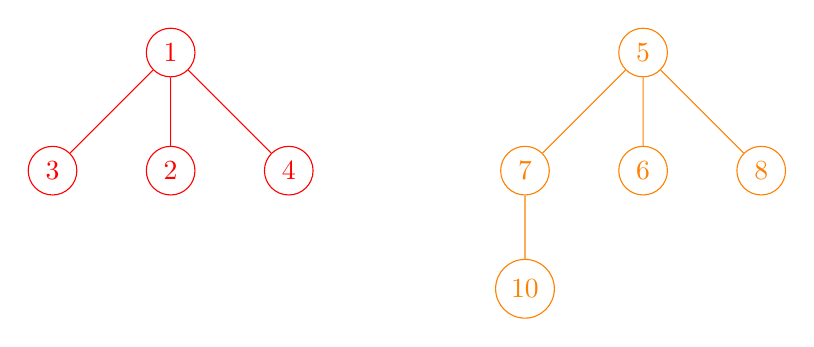
\begin{tikzpicture}
[  
    edge from parent/.style={thick}
]
    \begin{scope}[edge from parent/.style={draw=red}]
        \node [draw, circle, red] {1}
            child {node [draw, circle, red] {3}}
            child {node [draw, circle, red] {2}}
            child {node [draw, circle, red] {4}};
    \end{scope}
    
    \begin{scope}[edge from parent/.style={draw=orange}]
        \node [draw, circle, orange] at (6,0) {5}
            child {
                node [draw, circle, orange] {7}
                child {node [draw, circle, orange] {10}}
            }
            child {node [draw, circle, orange] {6}}
            child {node [draw, circle, orange] {8}};
    \end{scope}
\end{tikzpicture}
\end{center}

\end{frame}

\begin{frame}
\frametitle{Disjoint Set Union: Path Compression}

We can just unite root of the tree with the other one.

\begin{center}
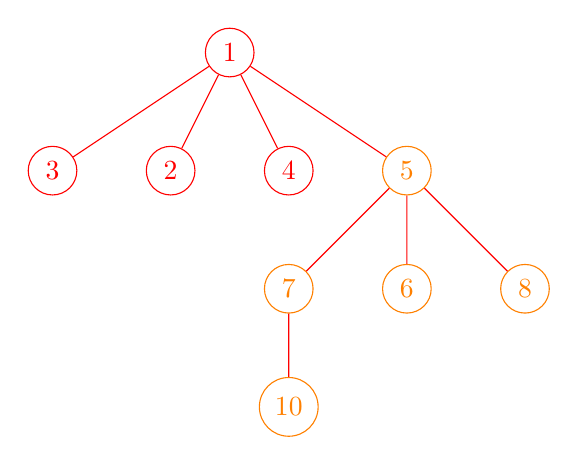
\begin{tikzpicture}
[  
    edge from parent/.style={draw=red}
]
    \node [draw, circle, red] {1}
        child {node [draw, circle, red] {3}}
        child {node [draw, circle, red] {2}}
        child {node [draw, circle, red] {4}}
        child {
            node [draw, circle, orange] {5} 
            child {
                node [draw, circle, orange] {7}
                child {node [draw, circle, orange] {10}}
            }
            child {node [draw, circle, orange] {6}}
            child {node [draw, circle, orange] {8}}
        };
\end{tikzpicture}
\end{center}

\end{frame}

\begin{frame}
\frametitle{Disjoint Set Union: Path Compression}

Call find\_root(7)

\begin{center}
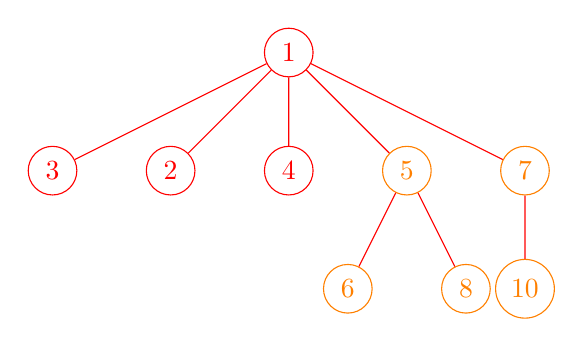
\begin{tikzpicture}
[  
    edge from parent/.style={draw=red}
]
    \node [draw, circle, red] {1}
        child {node [draw, circle, red] {3}}
        child {node [draw, circle, red] {2}}
        child {node [draw, circle, red] {4}}
        child {
            node [draw, circle, orange] {5} 
            child {node [draw, circle, orange] {6}}
            child {node [draw, circle, orange] {8}}
        }
        child {
            node [draw, circle, orange] {7}
            child {node [draw, circle, orange] {10}}
        };
\end{tikzpicture}
\end{center}

\end{frame}

\begin{frame}
\frametitle{Disjoint Set Union: Path Compression}

How about removing the last connection?

\begin{center}
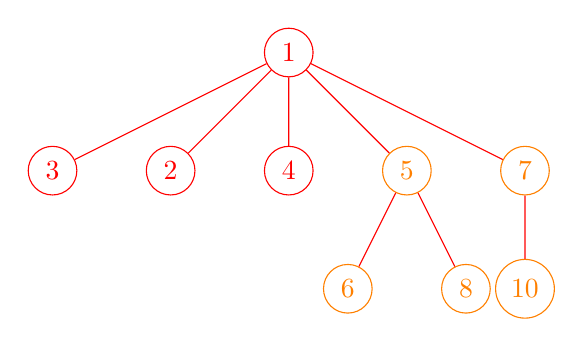
\begin{tikzpicture}
[  
    edge from parent/.style={draw=red}
]
    \node [draw, circle, red] {1}
        child {node [draw, circle, red] {3}}
        child {node [draw, circle, red] {2}}
        child {node [draw, circle, red] {4}}
        child {
            node [draw, circle, orange] {5} 
            child {node [draw, circle, orange] {6}}
            child {node [draw, circle, orange] {8}}
        }
        child {
            node [draw, circle, orange] {7}
            child {node [draw, circle, orange] {10}}
        };
\end{tikzpicture}
\end{center}

\end{frame}

\begin{frame}
\frametitle{Disjoint Set Union: Path Compression}

How about removing the last connection?

\begin{center}
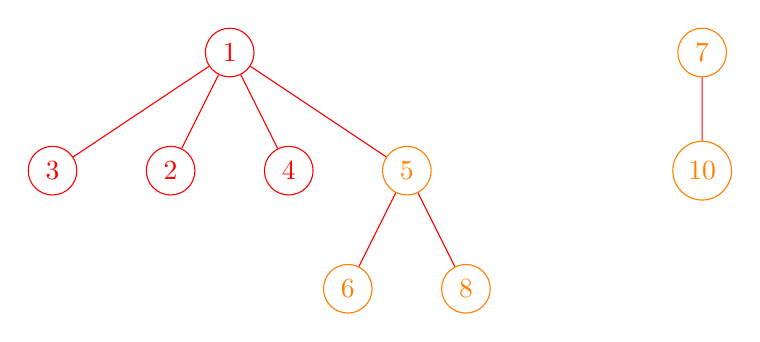
\begin{tikzpicture}
[  
    edge from parent/.style={draw=red}
]
    \node [draw, circle, red] {1}
        child {node [draw, circle, red] {3}}
        child {node [draw, circle, red] {2}}
        child {node [draw, circle, red] {4}}
        child {
            node [draw, circle, orange] {5} 
            child {node [draw, circle, orange] {6}}
            child {node [draw, circle, orange] {8}}
        };
    \node [draw, circle, orange] at (6, 0) {7}
        child {node [draw, circle, orange] {10}};
\end{tikzpicture}
\end{center}

But the tree is not the same!

\end{frame}

\begin{frame}
\frametitle{Disjoint Set Union: Path Compression}

Since path compression does not support removing the rollback, we need to use another approach.

\medskip

\centering
``Disjoint Set Union on Tree"

\begin{center}
    
\includegraphics[width=2cm]{devil.png}
\end{center}

\end{frame}